\chapter{Implementación}

Hasta ahora, con todas las piezas de información que hemos generado acerca del desarrollo, hemos podido, en efecto, discernir entre tres grandes grupos de tareas: la gestión, el calendario y el panel de control. Así pues, estableceremos la separación del desarrollo en estos tres grandes bloques de trabajo, con la previa especificación de las herramientas a utilizar y del trabajo anterior al comienzo del proceso de programación, propiamente dicho, que implican la puesta a punto de la base de datos y del servidor para probar y desarrollar nuestra aplicación.

\section{Herramientas para el desarrollo de twinX}

Como ya hemos mencionado en varias ocasiones, el desarrollo va a ser llevado a cabo con la ayuda de Yii2 Framework. En su segunda versión, este framework hace uso del lenguaje de programación PHP para orquestar múltiples tareas que resultan algo engorrosas de llevar a cabo sin su ayuda, como son, por ejemplo, las operaciones con la base de datos o la generación de código del que partir para dar forma a la vista, modelo o controlador de alguna de las secciones de twinX \cite{yii}.

Entre sus características, destacamos el generador de código Gii (figura \ref{fig:gii}), que puede automatizar la creación, por ejemplo, de la clase de un modelo, o incluso de una tabla CRUD al completo (esto es, su vista y su controlador). Tan solo tenemos que indicar cuál es la tabla de la base de datos sobre la que queremos generar los fragmentos de código, y atendiendo a las restricciones creadas en la misma, se puede obtener fácilmente una clase instanciable para recuperar o guardar información en su tabla. Del mismo modo, al crear una tabla CRUD, tendríamos directamente en nuestro sitio web una interfaz donde pueden verse los registros almacenados en la base de datos, con la posibilidad de crear nuevos, eliminarlos o incluso filtrarlos y editarlos. No cabe duda del potencial de esta característica, la cual nos permitirá ahorrar mucho tiempo y seguridad a la hora de desarrollar y de depositar la confianza en código automáticamente generado y sin errores.

\begin{figure}
	\centering
	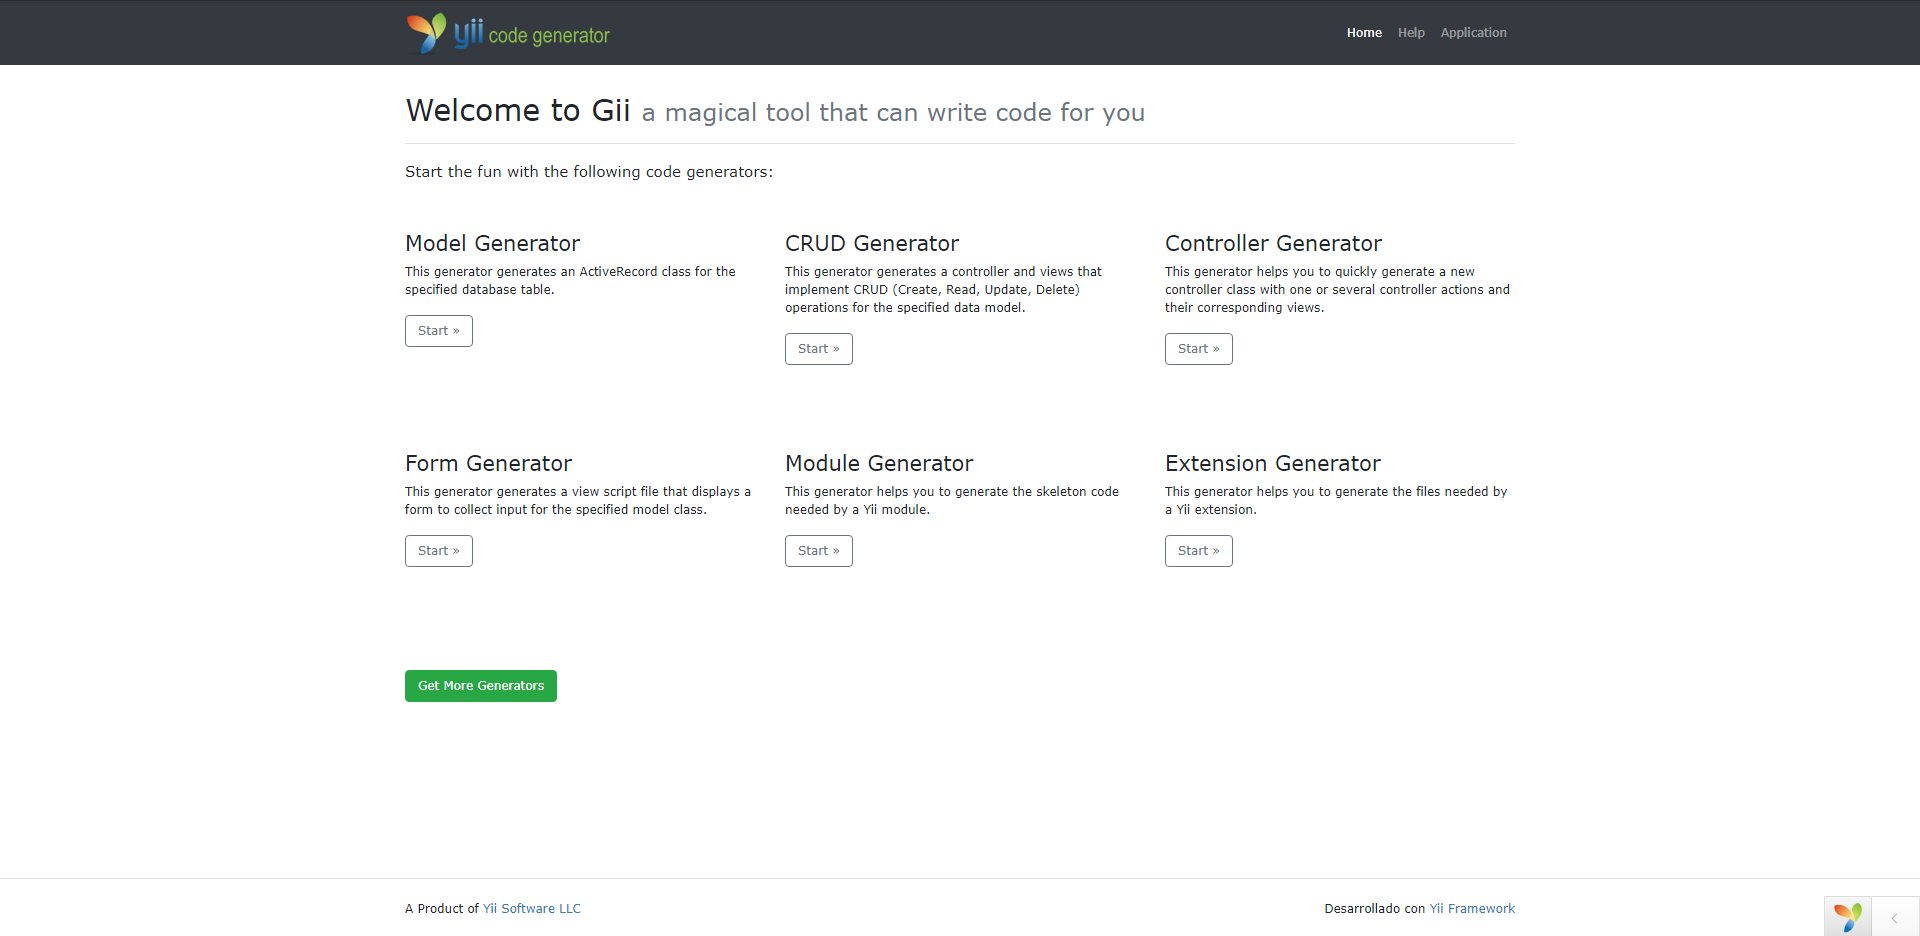
\includegraphics[width=\textwidth]{gii}
	\caption[Portal de Gii]{Portal de Gii desde donde podemos seleccionar un tipo de elemento a crear para que genere su código fuente}
	\label{fig:gii}
\end{figure}


Para comenzar a usar Yii, lo primero que tenemos que hacer es hacernos con el gestor de dependencias de PHP \textbf{Composer} \cite{composer} y descargarnos el esqueleto de un proyecto en Yii2 avanzado \cite{yii2advanced}. Para ello, basta con escribir:

\par\noindent\rule{\textwidth}{0.4pt}
\texttt{composer create-project --prefer-dist yiisoft/yii2-app-advanced twinX}
\smallskip

Y con ello ya tendríamos la carpeta con nuestro proyecto. Concretamente este directorio es el que tenemos que servir y al que nos conectaremos para visualizar nuestra web. También tenemos que seguir los pasos en el repositorio de GitHub de yiisoft para aplicar los ajustes necesarios derivados del renombramiento y redireccionamiento de URLs en el servidor. También tendremos que instalar algunas dependencias haciendo uso de la orden \texttt{composer install} y de iniciar el entorno de desarrollo con el archivo \texttt{ini} de PHP que incluye el repositorio que hemos clonado.

A continuación, procederemos con la instalación de la pila software \textbf{XAMPP} (Apache, MariaDB, PHP y Perl). En Windows, es una instalación sencilla a través de una interfaz de usuario, por lo que no requiere un gran tiempo. Es importante que, una vez instalado, situemos la carpeta del proyecto dentro del directorio \texttt{htdocs}, en la raíz de la carpeta de instalación de xampp. Se recomienda instalar en el directorio C:\ en Windows. En nuestro caso, hemos hecho los ajustes necesarios para poder situar esta carpeta en otro directorio desde donde se trabaja con el repositorio GitHub del proyecto, para que de forma más cómoda podamos salvaguardar el progreso del desarrollo de forma periódica sin tener que copiar archivos de un directorio que esté fuera del repositorio.

Esta pila contiene también la apliación \textbf{phpMyAdmin}, que ha sido también una gran ayuda para poder visualizar las tablas en base de datos, acceder a registros concretos o ejecutar código SQL desde una interfaz gráfica. Frente a una terminal desde donde manejar la base de datos, presenta una menor tasa de errores al introducir órdenes, pues la información puede verse a golpe de click y con una presentación más vistosa.

Sobre GitHub, al comienzo de la redacción de esta memoria se creó el repositorio \cite{repogit} donde, mediante la creación de ramas, hemos ido guardando en distintos commits las versiones del proyecto. Una vez creada una pieza de valor, se hacía una mezcla (\textit{merge}) a la rama \texttt{master}, de modo que cada rama se creaba con un fin, para añadir una nueva funcionalidad, sin depender del funcionamiento de las demás, para que poco a poco se puedan ir integrando las funcionalidades en su totalidad.

Finalmente, otro de los protagonistas del desarollo es el IDE (\textit{integrated development environment}) con que se ha programado twinX. En este caso, haciendo uso de su licencia educativa, se ha usado PhpStorm \cite{phpstorm}. Ha sido esencial, pues hemos descartado otras herramientas como Visual Studio Code ya que no tienen tan buen integración con PHP y Yii en sí como tiene este IDE. Destacan también características como su guardado automático inteligente, su potente búsqueda de archivos y sus cómodos atajos de teclado. Todo ello han hecho el proceso de desarrollo muy cómodo y liviano.


\section{Creación de la base de datos}



